\documentclass[10pt,conference]{IEEEtran}

% --- Packages ---
\usepackage[utf8]{inputenc}
\usepackage[T1]{fontenc}
\usepackage{booktabs}
\usepackage{hyperref}
\usepackage{amsmath}
\usepackage{amssymb}
\usepackage{graphicx}
\usepackage{xspace}
\usepackage{enumitem}
\usepackage{adjustbox}
\usepackage{dblfloatfix}

\hypersetup{
  colorlinks=true,
  linkcolor=blue,
  citecolor=blue,
  urlcolor=blue
}

\title{Which Context Surface Do LLMs Respect Most\\for Org-Specific Knowledge?\\
{\large An Evaluation Framework Using Controlled Retrieval Variants}}

\author{
  \IEEEauthorblockN{Srinivas Vaddi}
  \IEEEauthorblockA{Independent Researcher\\
  \href{https://github.com/vaddisrinivas/moltsnip}{github.com/vaddisrinivas/moltsnip}}
}

\begin{document}

\maketitle

\begin{abstract}
LLMs are surprisingly good at public coding benchmarks, yet surprisingly helpless the moment a task requires knowledge that was never in their training data.
Org-specific conventions --- the internal metrics API your team uses, the audit logging pattern that compliance requires, the exact error contract that downstream services depend on --- are invisible to a model that has only seen the public internet.
When a code repair task demands both a logic fix \emph{and} adherence to such a convention, the model must get that knowledge from somewhere.
The practical question is not \emph{whether} to provide it, but \emph{how}.

This paper introduces \textbf{Script30}, a pilot benchmark built around that question.
Thirty composition bugs --- each requiring a logic fix plus a call to the correct org-specific \texttt{orgops.*} function --- are evaluated under a seven-point context surface ladder (P0--P6) that isolates one delivery mechanism at a time, from no context at all to autonomous retrieval guided by \texttt{SKILL.md} and \texttt{AGENTS.md}.
Across two model families (\texttt{claude-haiku-4-5} and \texttt{gpt-5.1-codex-mini}, $n{=}3$ each, 1,229 scored runs), the results are striking and model-dependent.
For Haiku, autonomous retrieval with a focused guide document (P4, \textbf{69.2\%}) beat oracle injection (P3, \textbf{65.4\%}) and the unguided agentic baseline (P2, \textbf{39.7\%}).
For Codex, the ordering reversed: static injection (P3, \textbf{43.0\%}) substantially outperformed tool-based retrieval (P4, \textbf{20.0\%}).

These are directional findings from a small pilot.
The benchmark, harness, and all run artefacts are at \url{https://github.com/vaddisrinivas/moltsnip} (branch \texttt{arxiv-v1}).
\end{abstract}

\begin{IEEEkeywords}
large language models, code generation, retrieval-augmented generation, agentic coding, benchmark, org-specific knowledge, context surfaces, SKILL.md, AGENTS.md
\end{IEEEkeywords}

% ===================================================================
\section{Introduction}
\label{sec:introduction}

Suppose a developer asks a coding assistant to fix a bug in a cache eviction module.
The fix itself is straightforward: an off-by-one in a comparison operator.
But the task also requires calling \texttt{orgops.metrics.emit("cache.eviction",~utilization\_pct=pct)} --- a function from an internal metrics API that the model has never seen.
Without that call, the test fails.
The code is logically correct and policy-non-compliant simultaneously.

This scenario is not exotic. Any team that operates an LLM coding assistant for long enough will encounter it: a task where the model's training data has the algorithm but not the convention.
Public benchmarks such as HumanEval~\cite{chen2021evaluating} and SWE-bench~\cite{jimenez2024swebench} do not surface this class of failure because their tasks can, by construction, be solved from public knowledge.
The failure mode only becomes visible when correctness \emph{requires} adherence to org-specific policies absent from any public corpus.

When the model cannot infer the convention, it has to retrieve it.
The question for practitioners is: which retrieval mechanism is actually worth investing in?
Options range from manually curating per-task snippets and injecting them into the system prompt, to giving the model retrieval tools and hoping it searches effectively, to guiding that search with a \texttt{SKILL.md} or \texttt{AGENTS.md} document.
Each option has a different cost and a different payoff.

This paper reports an empirical attempt to measure those payoffs under controlled conditions.

The contributions are:

\begin{enumerate}
    \item \textbf{Script30 + P0--P6 ladder}: a 30-bug composition benchmark where each bug requires both a logic fix and an org-specific \texttt{orgops.*} call that models cannot infer from training data (P0 = 0.0\% on signal bugs), paired with a seven-point context surface ladder that varies exactly one delivery mechanism at a time, enabling clean absolute lift measurement against a zero baseline.
    \item \textbf{Pilot empirical observations} across two model families:
    for Haiku ($n{=}3$), autonomous retrieval with SKILL.md (P4$=$69.2\%) outperformed oracle injection (P3$=$65.4\%); for Codex ($n{=}3$), static injection (P3$=$43.0\%) substantially outperformed tool-based retrieval (P4$=$20.0\%).
    \item \textbf{A reproducible harness} with provider-parity controls, Docker-isolated pytest ground-truth scoring, per-run retrieval tracing, and published run artefacts.
\end{enumerate}

% ===================================================================
\section{Related Work}
\label{sec:related-work}

\textbf{Code generation benchmarks.}
HumanEval~\cite{chen2021evaluating}, MBPP~\cite{austin2021program}, and SWE-bench~\cite{jimenez2024swebench} measure model capability on public tasks.
This work differs in that correctness \emph{requires} adherence to org-specific conventions not reflected in training data, which eliminates training-data leakage as a competing explanation for success.

\textbf{Retrieval-augmented code generation.}
Prior work has shown that retrieval improves code generation~\cite{lewis2020retrieval}, including code-specific evaluations such as CodeRAG-Bench~\cite{wang2024coderagbench} and retrieval-policy studies~\cite{gu2025whattoretrieve}.
Documentation-grounded code generation has also been studied for API usage~\cite{chen2025apidocrag}.
The present setting differs by requiring org-specific policy conventions and by isolating \emph{how} context is delivered (injected vs.\ autonomous vs.\ guided) rather than whether retrieval helps at all.

\textbf{Context retrieval and guide surfaces for coding agents.}
Recent work benchmarks context retrieval behaviour in coding agents~\cite{cai2026contextbench} and studies repository-level guide files such as \texttt{AGENTS.md}~\cite{gloaguen2026agentsmd}.
Agent-skill benchmarks similarly evaluate how instruction packaging affects agent outcomes~\cite{li2026skillsbench}.
Script30 extends this line with a controlled P0--P6 ladder that directly compares \texttt{SKILL.md}-style guidance, \texttt{AGENTS.md}-style guidance, and their combination under fixed tasks and tools.

\textbf{Tool-augmented LLMs.}
Tool use has been studied in reasoning~\cite{schick2023toolformer}, web tasks~\cite{yao2023react}, and API-centric benchmarks~\cite{li2023apibank}, but less so in the specific setting of org-specific policy discovery during code repair.

\textbf{Agentic coding.}
SWE-agent~\cite{yang2024sweagent} and similar systems demonstrate multi-turn code repair.
Knowledge-layered approaches to program repair have also shown gains from structured context injection~\cite{ehsani2025hierarchical}.
This work complements that line by asking not \emph{can} agents repair bugs but \emph{which information channel} enables correct adherence to org-specific conventions.

% ===================================================================
\section{The Script30 Benchmark}
\label{sec:benchmark}

\subsection{Codebase}
\label{sec:codebase}

Script30 is built on a synthetic Python microservice codebase (\texttt{usecases/script30}) comprising approximately 2,000 lines of application source across six modules:

\begin{table}[t]
\centering
\caption{Script30 codebase modules.}
\label{tab:modules}
\begin{tabular}{@{}ll@{}}
\toprule
\textbf{Module} & \textbf{Domain} \\
\midrule
\texttt{cache/}  & Write-behind cache, TTL, LFU eviction \\
\texttt{data/}   & Migration runner, query scheduler \\
\texttt{logops/} & Log redaction, correlation ID propagation \\
\texttt{net/}    & DNS cache, retry policy, TLS validation \\
\texttt{errors/} & Circuit breaker, dead-letter queue \\
\texttt{orgops/} & Org policy: metrics, auditing, compliance \\
\bottomrule
\end{tabular}
\end{table}

The \texttt{orgops/} module is the \emph{information asymmetry surface}: it encodes org-specific policies through seven functions under the \texttt{orgops.*} namespace that are absent from any public corpus.
Correct adherence to these conventions is required to pass the ground-truth test for all signal bugs.

\subsection{Bug Construction}
\label{sec:bug-construction}

Each of the 30 bugs is a \textbf{composition bug}: passing the ground-truth test requires two independent fixes.

\begin{enumerate}
    \item \textbf{Logic fix} --- a deterministic code repair (e.g.\ invert a comparison operator, correct a modulo operand).
    \item \textbf{Policy-compliance fix} --- a call to the correct \texttt{orgops.*} function with the prescribed method name, event string, and keyword arguments.
\end{enumerate}

The logic fix is solvable from training data alone; the policy-compliance fix is not.
This structure ensures P0 cannot pass signal bugs while still requiring genuine reasoning for the logic component.

\textbf{Validity gating.}
Each bug satisfies three conditions: (a) P0 = 0 on signal bugs; (b) P3 oracle is non-zero; (c) the required snippet is retrievable from the VoltSnip corpus.

\subsection{Snippet Corpus}
\label{sec:snippet-corpus}

VoltSnip (a simple MCP/HTTP snippet store) serves \textbf{35 snippets} for Script30: 5 guiding-principle snippets (one per bug category) and 30 scenario-context snippets (one per bug), each containing the specific \texttt{orgops.*} convention, expected arguments, and a correct usage example.
Each task declares exactly two required snippets.
During dynamic retrieval (P4--P6), the model may retrieve up to 4 snippets per query.

% ===================================================================
\section{The Context Surface Ladder}
\label{sec:ladder}

The central design decision in Script30 is the ladder: seven \textbf{hypothesis variants} (P0--P6) that each vary exactly one dimension of context delivery, making lift measurements attributable to the one thing that changed.

\begin{table}[t]
\centering
\caption{Context surface ladder (P0--P6). ``Guide type'' indicates which
  guidance document's \emph{content} is active; in all agentic variants
  (P4--P6) the same content is also written to \texttt{CLAUDE.md},
  which Claude Code reads automatically.}
\label{tab:ladder}
\small
\begin{tabular}{@{}lllll@{}}
\toprule
\textbf{Var.} & \textbf{Surface} & \textbf{Tools} & \textbf{Retrieval} & \textbf{Guide type} \\
\midrule
P0 & None (baseline)       & $\times$   & None      & ---        \\
P1 & Instruction framing   & $\times$   & None      & ---        \\
P2 & Tools only            & \checkmark & Agent     & ---        \\
P3 & Oracle injection      & $\times$   & Injected  & ---        \\
P4 & Focused guide + tools & \checkmark & Agent     & SKILL.md   \\
P5 & Alt.\ guide + tools   & \checkmark & Agent     & AGENTS.md  \\
P6 & Both guides + tools   & \checkmark & Agent     & Both       \\
\bottomrule
\end{tabular}
\end{table}

\textbf{P0} anchors all measurements: the model sees only the bug description, the target file, and a generic repair instruction.
\textbf{P1} adds explicit instruction framing without any org-specific knowledge; it tests whether careful prompting alone helps.
\textbf{P2} (agentic baseline) provides retrieval tools with no guide; P4$-$P2 measures the marginal value of a focused guide.
\textbf{P3} (oracle) pre-injects the exact required snippets and provides an upper-bound estimate of what correct context is worth.
\textbf{P4--P6} are the autonomous retrieval variants.
The SKILL-style guide (P4) is a focused retrieval guide (4,330\,chars) that
defines MCP tool semantics, query-construction rules, and a step-by-step
retrieval workflow for bug-fix tasks~\cite{li2026skillsbench}.
The AGENTS-style guide (P5) is an agent workflow guide (3,821\,chars)
covering agent priorities, retrieval decision rules, and MCP failure
handling~\cite{gloaguen2026agentsmd}.
Both withhold snippet keys; the model must formulate queries from task context.
P6 receives both guides simultaneously.
Guide delivery relies on Claude Code's native \texttt{CLAUDE.md} and
\texttt{AGENTS.md} auto-loading from the per-run working directory (not
tool calls; \texttt{Read}/\texttt{Glob}/\texttt{Grep} are in
\texttt{--disallowedTools}): in P4 both \texttt{CLAUDE.md} and
\texttt{AGENTS.md} carry the SKILL-style content; in P5 both carry
the AGENTS-style content; in P6 \texttt{CLAUDE.md} and \texttt{AGENTS.md}
carry the AGENTS-style content while a \texttt{SKILL.md} file is also
present (accessible only if the model explicitly requests it, which
\texttt{--disallowedTools} prevents).
The formal variant specification is in Appendix~\ref{app:variant-spec}.

% ===================================================================
\section{Evaluation Harness}
\label{sec:harness}

\subsection{Provider Parity}
\label{sec:provider-parity}

Both models---\textbf{claude-haiku-4-5} (Claude Code CLI) and \textbf{gpt-5.1-codex-mini} (Codex CLI)---are configured for maximum parity across four dimensions.

\textbf{Tools.} Both see only VoltSnip MCP tools (7 endpoints: search,
read-by-key, semantic search, and view variants); the two primary tools
are \texttt{search\_memory} (discovery) and
\texttt{get\_snippet\_by\_canonical\_key} (precision retrieval).
Filesystem tools are excluded from both.

\textbf{Isolation.} Both run with \texttt{cwd} set to a fresh per-run tmpdir.
Claude Code blocks \texttt{Bash}, \texttt{Edit}, \texttt{Write}, \texttt{Read}, \texttt{Glob}, and \texttt{Grep} via \texttt{--disallowedTools}; Codex runs with \texttt{--sandbox read-only} and global MCP servers wiped.

\textbf{Tool budget.} Tool-enabled variants (P2, P4--P6) are capped at
\texttt{max\_tool\_roundtrips=4}, enforced by injecting
``Maximum tool roundtrips: 4'' into the user-visible prompt section;
no CLI \texttt{--max-turns} flag is used, so the model self-limits
based on the stated budget.

\textbf{Residual asymmetry.} Each provider retains a secondary read surface (Codex via sandbox; Claude Code via \texttt{ReadMcpResourceTool}).
The \texttt{cwd=tmpdir} boundary isolates both from \texttt{orgops/}.
P0 = 0.0\% on signal bugs for both providers confirms this held in practice.

\subsection{Scoring}
\label{sec:scoring}

\textbf{Primary: pytest pass rate.}
Each patch is applied to a Docker overlay of the target repository and the task's pytest test runs in a network-isolated container (300\,s timeout).
A run passes if and only if pytest exits 0.
Each test verifies both the logic fix and the correct \texttt{orgops.*} call signature via \texttt{unittest.mock.patch}.

\textbf{Secondary: LLM judge.}
A \texttt{gpt-5.2} judge with structured checks~\cite{li2024llmjudge} is reported for reference only; it inflates pass rates by approximately 15--25\,pp relative to pytest.
All primary claims use pytest.

\subsection{Validity Gating and Retrieval Tracing}
\label{sec:validity}

Three invariants prevent bad runs from entering results:
\texttt{status=ok} runs with no generated code are demoted to error;
Claude Code \texttt{is\_error=true} stream events are raised as provider errors;
on resume, error runs are retried rather than cached.

Each task specifies \texttt{required\_snippet\_keys}.
The harness records per-run coverage, hit/missing keys, and retrieved-key precision.
\textbf{Full coverage} (\texttt{coverage=1.0}) is the primary retrieval metric.
P3 snippets are injected directly and marked fully covered by construction.

% ===================================================================
\section{Experimental Setup}
\label{sec:setup}

\begin{table}[t]
\centering
\caption{Models evaluated and run counts.}
\label{tab:models}
\small
\begin{tabular}{@{}llcr@{}}
\toprule
\textbf{Provider} & \textbf{Model} & \textbf{$n$} & \textbf{Scored} \\
\midrule
Claude Code & claude-haiku-4-5   & 3 & 630 \\
Codex       & gpt-5.1-codex-mini & 3 & 599 \\
\bottomrule
\end{tabular}
\end{table}

Haiku completed the full 30-bug $\times$ 7-variant matrix (630 cells, 0 errors).
Codex had provider errors in some cells (Run~1: 30/210; Run~2: 0; Run~3: 1/210), which were excluded from scoring.
The 1,229 scored runs (630 Haiku + 599 Codex) exclude error-status cells.

VoltSnip serves 35 snippets via a hosted MCP server.
Snippet code fields are truncated to 1,200 characters uniformly across all variants that use snippets (P3--P6).

% ===================================================================
\section{Results}
\label{sec:results}

\textbf{Pass rate} is the fraction of scored runs where pytest exits 0; \textbf{lift} is the absolute percentage-point (pp) gain over P0 (see Appendix~\ref{app:metrics}).
Since P0 = 0.0\% on signal bugs for Haiku, lift equals pass rate directly for that model.

\subsection{Observed Surface Ordering}
\label{sec:surface-hierarchy}

\begin{table}[t]
\centering
\caption{Pass rates --- Haiku (26 signal bugs, $n{=}3$).}
\label{tab:results-haiku}
\small
\begin{tabular}{@{}lcr@{}}
\toprule
\textbf{Variant} & \textbf{Pass rate} & \textbf{Lift} \\
\midrule
P0 & 0.0\% (0/78)    & ---         \\
P1 & 2.6\% (2/78)    & $+$2.6 pp   \\
P2 & 39.7\% (31/78)  & $+$39.7 pp  \\
P3 & 65.4\% (51/78)  & $+$65.4 pp  \\
P4 & \textbf{69.2\%} (54/78) & $+$69.2 pp \\
P5 & 67.9\% (53/78)  & $+$67.9 pp  \\
P6 & 60.3\% (47/78)  & $+$60.3 pp  \\
\bottomrule
\end{tabular}
\end{table}

\begin{table}[t]
\centering
\caption{Pass rates --- Codex (30 bugs, $n{=}3$, errors excluded).}
\label{tab:results-codex}
\small
\begin{tabular}{@{}lcr@{}}
\toprule
\textbf{Variant} & \textbf{Pass rate} & \textbf{Lift} \\
\midrule
P0 & 4.7\% (4/86)    & ---         \\
P1 & 5.9\% (5/85)    & $+$1.2 pp   \\
P2 & 26.7\% (23/86)  & $+$22.0 pp  \\
P3 & \textbf{43.0\%} (37/86) & $+$38.3 pp \\
P4 & 20.0\% (17/85)  & $+$15.3 pp  \\
P5 & 24.4\% (21/86)  & $+$19.7 pp  \\
P6 & 30.6\% (26/85)  & $+$25.9 pp  \\
\bottomrule
\end{tabular}
\end{table}

\emph{Note: Haiku results use the 26-bug signal set (excluding 4 noisy bugs where P0 passes stochastically). Codex results use all 30 bugs; the signal set has not been validated with the same noisy-bug analysis. All-bugs results for Haiku are in Appendix~\ref{app:all-bugs}.}

The results tell two different stories. For Haiku, the hierarchy is clean: providing retrieval tools helps substantially ($+$39.7~pp over P0), a focused guide helps further, and the guide-plus-tools combination (P4, 69.2\%) edges out even the oracle that pre-injects the exact correct snippets (P3, 65.4\%). For Codex, the story reverses: oracle injection is the best condition, and tool-based retrieval performs poorly.

\begin{figure}[t]
\centering
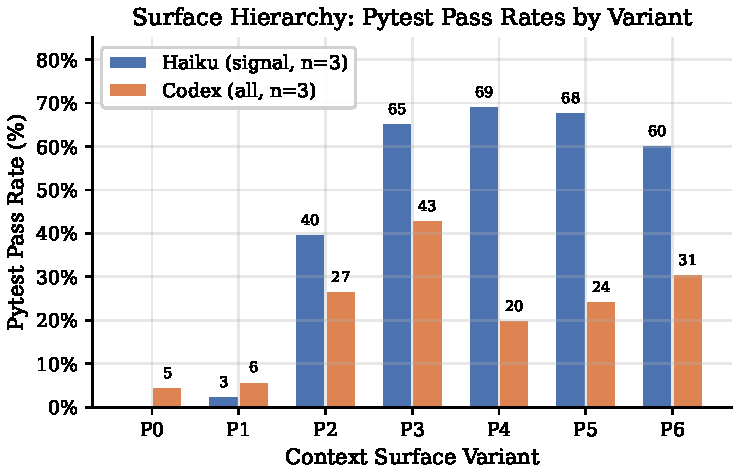
\includegraphics[width=\columnwidth]{figures/fig1_surface_hierarchy.pdf}
\caption{Pass rates by context surface variant. P4 is the top Haiku variant; P3 is the top Codex variant. The two models are on different bug sets and are not directly comparable.}
\label{fig:surface-hierarchy}
\end{figure}

\subsection{Causal Attribution}
\label{sec:causal-attribution}

Four conditions confirm that P4's lift is retrieval-dependent:

\begin{enumerate}
    \item P0 = 0.0\% on all 26 signal bugs --- training data cannot produce the org convention. \checkmark
    \item \texttt{voltsnip\_tool\_call\_count} $>$ 0 for all passing P4 runs. \checkmark
    \item \texttt{native\_tool\_call\_count} $=$ 0 for P4 runs --- no filesystem tools used. \checkmark
    \item P4 drops to 0.0\% when VoltSnip returns no snippets (ablation below). \checkmark
\end{enumerate}

\textbf{Empty-store ablation.}
One Haiku P4 run ($n{=}1$, 26 signal bugs) was conducted with all VoltSnip snippets hidden via \texttt{is\_hidden=true}.
The model retained the SKILL.md guide and tools; queries succeeded but returned zero results.
Pass rate: \textbf{0.0\%} (0/26) versus 69.2\% for the standard P4 condition.
Guide framing alone, without retrievable content, does not account for the observed lift.

\begin{figure}[t]
\centering
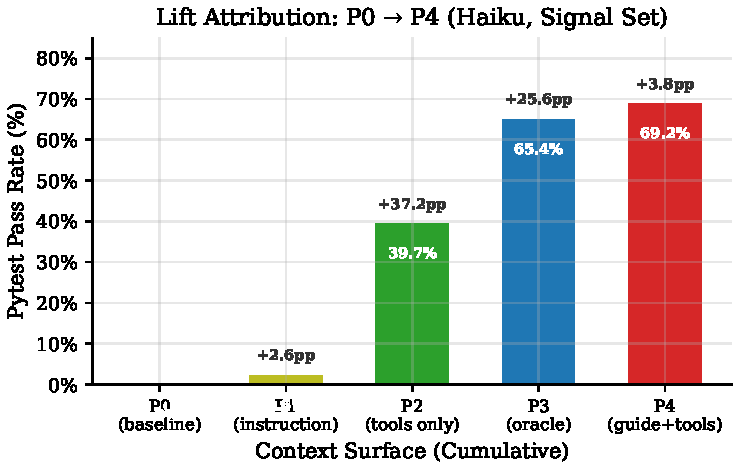
\includegraphics[width=\columnwidth]{figures/fig3_lift_waterfall.pdf}
\caption{Cumulative lift from P0 to P4 for Haiku (26 signal bugs). Each bar shows absolute pass rate; annotations show incremental lift from the previous variant.}
\label{fig:lift-waterfall}
\end{figure}

\subsection{Over-Specification Effect (P6 $<$ P4)}
\label{sec:over-specification}

P6 (both guides + tools, 60.3\%) scored 8.9~pp below P4 (SKILL.md only, 69.2\%) for Haiku.
Retrieval quality analysis explains the mechanism: P6 achieved full coverage (both required snippets retrieved) in only 22.2\% of runs versus 36.1\% for P4.
Yet when P6 \emph{did} achieve full coverage, it passed 100.0\% of the time (vs.\ 92.3\% for P4).
P6 is not worse at applying retrieved knowledge; it is worse at retrieving it.
Having two guide documents with overlapping directives appears to degrade query formulation, consistent with findings on competing context~\cite{liu2023lostmiddle}.
At $n{=}3$ with P4's inter-run range of 26.9~pp (Table~\ref{tab:per-run}), the 8.9~pp gap is not statistically confirmed, but the retrieval mechanism is mechanically traceable.

\subsection{Cross-Model Divergence}
\label{sec:cross-model}

\begin{table}[t]
\centering
\caption{Cross-model comparison (approximate; different bug sets).}
\label{tab:cross-model}
\small
\begin{tabular}{@{}lccc@{}}
\toprule
\textbf{Variant} & \textbf{Haiku} & \textbf{Codex} & $\boldsymbol{\Delta}$ \\
\midrule
P0                     & 0.0\%  & 4.7\%  & $-$4.7 pp  \\
P3 (oracle)            & 65.4\% & \textbf{43.0\%} & $+$22.4 pp \\
P4 (SKILL.md + tools)  & \textbf{69.2\%} & 20.0\% & $+$49.2 pp \\
P5 (AGENTS.md + tools) & 67.9\% & 24.4\% & $+$43.5 pp \\
P6 (both + tools)      & 60.3\% & 30.6\% & $+$29.7 pp \\
\bottomrule
\end{tabular}
\end{table}

For Codex, the highest-scoring variant (P3$=$43.0\%) uses no tools.
Codex P3 was stable across runs (range 10~pp: 36.7--46.7\%), while Codex P4 collapsed in two of three runs (Run~1: 46.2\%, Run~2: 6.7\%, Run~3: 10.0\%) --- a 40~pp swing.
Retrieval quality analysis shows Codex P4 achieved full-coverage retrieval in only 3.6\% of runs versus 36.1\% for Haiku P4, pointing to a tool-use issue rather than a stable model preference.

\subsection{Per-Run Variance (Haiku)}
\label{sec:variance}

\begin{table}[t]
\centering
\caption{Per-run pass rates, Haiku (26 signal bugs).}
\label{tab:per-run}
\small
\begin{tabular}{@{}lccccc@{}}
\toprule
\textbf{Var.} & \textbf{R1} & \textbf{R2} & \textbf{R3} & \textbf{Mean} & \textbf{Range} \\
\midrule
P0 & 0.0\%  & 0.0\%  & 0.0\%  & 0.0\%  & 0 pp    \\
P2 & 30.8\% & 42.3\% & 46.2\% & 39.7\% & 15.4 pp \\
P3 & 61.5\% & 69.2\% & 65.4\% & 65.4\% & 7.7 pp  \\
P4 & 57.7\% & 84.6\% & 65.4\% & 69.2\% & 26.9 pp \\
P6 & 65.4\% & 61.5\% & 53.8\% & 60.3\% & 11.6 pp \\
\bottomrule
\end{tabular}
\end{table}

P4 shows the widest range (26.9~pp), reflecting stochastic retrieval strategy across runs.
P3 is tighter (7.7~pp) because injected context is deterministic.
P0 is perfectly stable at 0.0\%, confirming the zero-leakage design.
Run~1 is notable: P3 (61.5\%) outperformed P4 (57.7\%), a reminder that P4 $>$ P3 in aggregate does not hold in every run.

\begin{figure}[t]
\centering
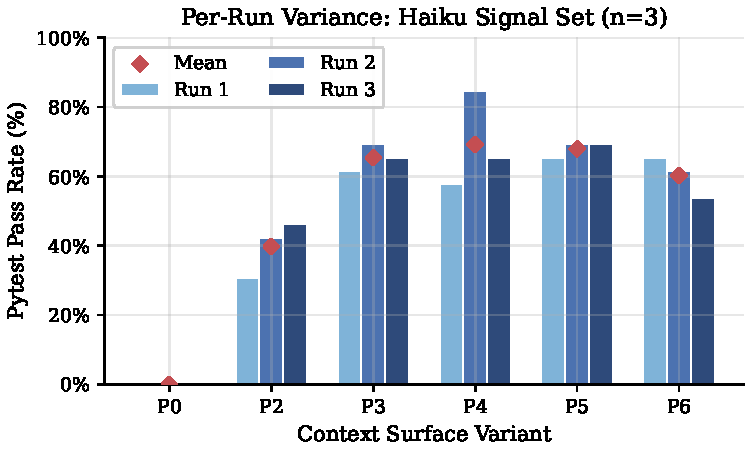
\includegraphics[width=\columnwidth]{figures/fig2_per_run_variance.pdf}
\caption{Per-run pass rates for Haiku (26 signal bugs). P4 has the widest inter-run variance (26.9~pp); P0 is stable at 0.0\%.}
\label{fig:per-run-variance}
\end{figure}

% ===================================================================
\section{Analysis and Discussion}
\label{sec:discussion}

\subsection{Why Autonomous Retrieval May Beat Oracle Injection}
\label{sec:p4-vs-p3}

The aggregate result that P4 (69.2\%) $\geq$ P3 (65.4\%) for Haiku is interesting but needs careful interpretation.
P3 injects the exact correct snippets; P4 requires the model to find them.
Naively, P3 should win.

Two explanations are plausible.
The retrieval-cueing hypothesis holds that the act of searching prompts the model to attend more carefully to retrieved content.
A better-supported explanation is that SKILL.md provides value beyond cueing: it frames \emph{how} to apply retrieved knowledge, not just \emph{what} to retrieve.

Supporting this: passing P4 runs ($N{=}54$) used a mean of 1.4 VoltSnip tool calls versus 0.7 for failing runs ($N{=}24$).
P2 (tools, no guide) also passes at 89.5\% when it achieves full coverage --- nearly as high as P4 (92.3\%) --- but P2 achieves full coverage in only 26.4\% of runs versus 36.1\% for P4.
The guide's main effect is raising retrieval success rate, not improving interpretation of already-available content.

\subsection{Why More Guidance Can Hurt}
\label{sec:guide-effects}

SKILL.md (P4) scored slightly higher than AGENTS.md (P5), and both outperformed their combination (P6).
The over-specification effect in Section~\ref{sec:over-specification} suggests a simple model: guide documents direct retrieval attention, but stacking two overlapping directives degrades query formulation.
This aligns with SkillsBench's finding that focused skills outperform comprehensive documentation~\cite{li2026skillsbench}.

\subsection{The Codex Divergence}
\label{sec:codex-divergence}

Codex's preference for static injection over dynamic retrieval may reflect: (1) lower tool-use proficiency; (2) MCP integration maturity (the Codex HarnessMCPServer uses HTTP URL-based transport; protocol edge cases required compliance work); or (3) a multi-run effect (Runs~2--3 both collapsed on tool variants, making a transient explanation less likely).

The cross-model divergence is the most practically important finding in this paper.
If it holds at larger $n$, the right deployment strategy is model-dependent: Haiku-class models may be ready for autonomous retrieval; Codex-class models may need curated injection until their tool-use matures.

\subsection{Tentative Implications for Practitioners}
\label{sec:implications}

If the Haiku hierarchy (P4 $>$ P5 $>$ P3 $>$ P6 $>$ P2 $>$ P1 $\approx$ P0) holds at larger $n$:

\begin{itemize}
    \item \textbf{Retrieval tooling matters far more than prompt engineering.} Gap P4 $-$ P1 $=$ $+$66.6~pp; careful framing without retrieval adds almost nothing ($+$2.6~pp).
    \item \textbf{One focused guide may be enough.} P4 outperformed P6 by 8.9~pp, though not statistically confirmed at $n{=}3$.
    \item \textbf{Autonomous retrieval may eliminate the need for oracle injection.} P4 (69.2\%) scored comparably to P3 (65.4\%); oracle injection requires upfront human curation of per-task snippets, expensive at scale.
    \item \textbf{Verify tool-use before relying on it.} Codex P4 was highly variable (range 40~pp) while P3 was stable (range 10~pp), pointing to a tool-use issue that practitioners should measure on their own model.
\end{itemize}

\subsection{Failure Mode Analysis}
\label{sec:qualitative}

Inspection of tool traces and model outputs reveals four recurring failure patterns:

\begin{enumerate}
    \item \textbf{Convention omission (P0--P1).} Models produce logically correct fixes but omit the \texttt{orgops.*} call or substitute a plausible stub. Dominant failure at P0--P1.
    \item \textbf{Tool avoidance (P2, P6).} Models skip tool calls and attempt a direct fix, even with tools available. SKILL.md substantially reduces this.
    \item \textbf{Poor query formulation (P2, P6).} Overly broad queries (\texttt{"metrics"}) return unrelated snippets. P4's 36.1\% full-coverage rate versus P2's 26.4\% reflects the guide improving query targeting.
    \item \textbf{Retrieved-but-misapplied (rare, $\sim$7.7\% of P4 full-coverage failures).} Both snippets retrieved, fix still fails --- wrong keyword argument name (\texttt{pct=} instead of \texttt{utilization\_pct=}) or wrong call site.
\end{enumerate}

Failure modes 2--3 (retrieval failures) are the primary bottleneck at P2 and P6. Mode 4 (application failure) is rare and only visible once retrieval is working.

% ===================================================================
\section{Limitations}
\label{sec:limitations}

\begin{enumerate}
    \item \textbf{Benchmark construction.} Built by the author with full knowledge of bugs and snippets; no third-party validation. Mitigations: P0$=$0 and P3$>$0 checks per bug; four noisy bugs excluded with documented rationale; Docker-isolated pytest scoring. Benchmark tests composition execution (fix bug + apply retrieved convention), not bug discovery; logic errors are marked inline.

    \item \textbf{Snippet fidelity.} Each scenario snippet provides the exact \texttt{orgops.*} call --- near-complete specification of the fix. Real org knowledge bases are more abstract. This inflates absolute pass rates for P3--P6 relative to production, but does not affect the P3 vs.\ P4 comparison (identical content; delivery is the only variable).

    \item \textbf{Scoring precision.} Pytest checks exact keyword argument names (\texttt{utilization\_pct=}, not \texttt{pct=}) --- by design, testing precise adherence to retrieved guidance.

    \item \textbf{Uniform difficulty labels.} All tasks labelled \texttt{difficulty: hard} with uncalibrated \texttt{trap\_baseline=0.15}, despite difficulty ranging from a single-character fix (BUG42) to recursive traversal with base64 decoding (BUG70). Snippet code fields are truncated to 1,200 characters; 12 snippets lose trailing content, but \texttt{orgops.*} details are preserved for all 12.

    \item \textbf{Scale and corpus.} $n{=}3$ is small. The 35-snippet corpus understates real retrieval difficulty, though corpus size is fixed across variants so relative comparisons remain valid.

    \item \textbf{Single codebase and language.} All 30 bugs are in one synthetic Python repository. Generalisability to other languages or real codebases is not established.

    \item \textbf{Residual provider asymmetry.} Each provider retains a secondary read surface. P0$=$0.0\% for both is consistent with isolation holding, but cross-provider comparisons carry this caveat.
\end{enumerate}

% ===================================================================
\section{Future Work}
\label{sec:future-work}

Priority extensions: (1) more model families (Sonnet/Opus, GPT-5.2-Codex, open-weight) to test whether the surface hierarchy generalises; (2) more Codex runs ($n{=}5+$) to distinguish infrastructure instability from a stable tool-use limitation; (3) abstract snippets providing principle-level guidance instead of per-bug specs, closer to production; (4) larger corpus (35 $\to$ 500+ snippets with distractors); (5) difficulty tiers and negative controls (tasks with no applicable \texttt{orgops.*} convention); (6) other languages (TypeScript, Java, Go); (7) guide style ablation (minimal vs.\ verbose, directive vs.\ suggestive); (8) hermetic Docker-layer isolation for both providers; (9) per-bug retrieval traces to cleanly separate ``never retrieved'' from ``retrieved but not applied.''

% ===================================================================
\section{Conclusion}
\label{sec:conclusion}

LLMs fail predictably on code tasks that require org-specific conventions absent from their training data.
Script30 is a 30-bug composition benchmark, paired with a seven-point context surface ladder (P0--P6), designed to measure that failure and the effect of different strategies for addressing it.

Three findings stand out.
First, \textbf{retrieval works dramatically}: Haiku's P4 (69.2\%) improves pass rate by 69.2~pp over the no-context baseline (P0, 0.0\%), and an empty-store ablation confirms the lift is retrieval-dependent.
Second, \textbf{more guidance is not always better}: P6 (60.3\%) underperforms P4 (69.2\%) because two overlapping guide documents degrade retrieval query formulation (22.2\% vs.\ 36.1\% full-coverage rate), not application.
Third, \textbf{the right strategy is model-dependent}: Haiku's autonomous retrieval beat oracle injection in aggregate; Codex's static injection was stable while tool-based retrieval collapsed in two of three runs.

These are pilot findings at $n{=}3$, one Python codebase, two models.
The benchmark and harness are reusable across models and retrieval backends.
All code, run artefacts, and analysis scripts are at \url{https://github.com/vaddisrinivas/moltsnip} (branch \texttt{arxiv-v1}).

% ===================================================================
\bibliographystyle{IEEEtran}
\bibliography{references}

% ===================================================================
\appendix

\section{Variant Ladder Formal Specification}
\label{app:variant-spec}

\begin{table}[t]
\centering
\caption{Formal specification of the seven hypothesis variants.}
\label{tab:variant-spec}
\footnotesize
\begin{adjustbox}{max width=\columnwidth}
\begin{tabular}{@{}llllllll@{}}
\toprule
\textbf{Field} & \textbf{P0} & \textbf{P1} & \textbf{P2} & \textbf{P3} & \textbf{P4} & \textbf{P5} & \textbf{P6} \\
\midrule
\texttt{mode}          & dir. & dir. & agent & agent & agent & agent & agent \\
\texttt{memory}        & $\times$ & $\times$ & $\times$ & \checkmark & $\times$ & $\times$ & $\times$ \\
\texttt{tools}         & $\times$ & $\times$ & \checkmark & $\times$ & \checkmark & \checkmark & \checkmark \\
\texttt{retrieval}     & none & none & agent & inject & agent & agent & agent \\
\texttt{instruction}   & none & expl. & none & none & none & none & none \\
\texttt{surface}       & user & user & tools & sys & skill & agents & both \\
\texttt{max\_trips}    & 1 & 1 & 4 & 4 & 4 & 4 & 4 \\
\bottomrule
\end{tabular}
\end{adjustbox}
\end{table}

\section{All-Bugs Results (Haiku, $n{=}3$)}
\label{app:all-bugs}

\begin{table}[t]
\centering
\caption{Pass rates on all 30 bugs (Haiku, $n{=}3$).}
\label{tab:all-bugs}
\small
\begin{tabular}{@{}lcr@{}}
\toprule
\textbf{Variant} & \textbf{Pass rate} & \textbf{Lift} \\
\midrule
P0 & 5.6\% (5/90)   & ---         \\
P1 & 6.7\% (6/90)   & $+$1.1 pp   \\
P2 & 42.2\% (38/90) & $+$36.6 pp  \\
P3 & 65.6\% (59/90) & $+$60.0 pp  \\
P4 & 71.1\% (64/90) & $+$65.5 pp  \\
P5 & 71.1\% (64/90) & $+$65.5 pp  \\
P6 & 61.1\% (55/90) & $+$55.5 pp  \\
\bottomrule
\end{tabular}
\end{table}

\emph{Includes the 4 noisy bugs (BUG41, BUG59, BUG62, BUG68) where P0 passes stochastically. P4 and P5 tie at 71.1\% in the all-bugs set despite P4 (69.2\%) $>$ P5 (67.9\%) on signal bugs; noisy bugs slightly favour P5.}

\section{Harness Integrity Fixes}
\label{app:harness-fixes}

Three bugs were discovered and corrected during the study:
(1) \textbf{Stream error detection} (\texttt{claudecode.py}): \texttt{is\_error=true} events were silently producing \texttt{status=ok} runs with empty code; fixed by adding a stream error extractor.
(2) \textbf{Empty-output gate} (\texttt{runner.py}): runs with \texttt{status=ok} but no code were not demoted to error; fixed by post-run validity check.
(3) \textbf{Resume integrity} (\texttt{csv\_mapper.py}): \texttt{load\_completed} loaded all entries regardless of status; fixed by filtering to \texttt{status=ok}.
All affected runs were re-executed after fixes were applied.

\section{Artefact Paths}
\label{app:artefacts}

All run artefacts are at \url{https://github.com/vaddisrinivas/moltsnip} (branch \texttt{arxiv-v1}), subdirectory \texttt{vsevals\_runs/batch\_1/}.
Every quantitative claim is mechanically derived from the CSV artefacts via \texttt{scripts/build\_paper.py};
running \texttt{uv run python3 scripts/build\_paper.py --check} reproduces all numbers from the raw CSVs.

\begin{table}[t]
\centering
\caption{Key artefact locations (paths relative to \texttt{vsevals/}).}
\label{tab:artefacts}
\footnotesize
\begin{tabular}{@{}ll@{}}
\toprule
\textbf{Artefact} & \textbf{Path} \\
\midrule
Suite definition     & \texttt{suites/script30.yaml} \\
Task definitions     & \texttt{tasks/script30/BUG\{41..70\}.yaml} \\
Snippet corpus       & \texttt{snippets/script30/} \\
Usecase codebase     & \texttt{usecases/script30/} \\
Pytest tests         & \texttt{usecases/script30/tests/unit/} \\
Haiku Runs 1--3      & \texttt{.../batch\_1/matrix\_20260303T19*} \\
Codex Runs 1--3      & \texttt{.../batch\_1/matrix\_20260303T19*, ...T20*, ...T08*} \\
Ablation (empty)     & \texttt{.../batch\_1/matrix\_20260304T095907*} \\
Build/check script   & \texttt{scripts/build\_paper.py} \\
\bottomrule
\end{tabular}
\end{table}

\section{Metric Definitions}
\label{app:metrics}

\textbf{Pass rate} for variant $v$ over bug set $B$ with $n$ valid runs:
\[
  \text{pass\_rate}(v) = \frac{\text{\# pytest-passed cells}}{\lvert B \rvert \times n}
\]
Cells with \texttt{status$\neq$ok} are excluded from numerator and denominator.

\textbf{Lift}: $\text{lift}(v) = \text{pass\_rate}(v) - \text{pass\_rate}(\text{P0})$, in percentage points (not a relative ratio).

\section{Inference Parameters and Training Data}
\label{app:model-details}

Both providers used CLI defaults; no temperature override was applied.
\textbf{claude-haiku-4-5} and \textbf{gpt-5.1-codex-mini} both have training data cutoffs of approximately early 2025.
The \texttt{orgops.*} API was constructed specifically for this benchmark, never published, and postdates both models' cutoffs.
Neither model was fine-tuned on the Script30 codebase.
P0$=$0.0\% on signal bugs (Haiku, all three runs) provides empirical confirmation of zero leakage.

\end{document}
